\chapter{Detection and classification}
\label{ch:methods}

\newthought{We now present a novel graphical method} for detecting and classifiying \textit{de novo} variants.  We shall briefly present the workings of the algorithms, relying on the \textit{de novo} assembly foundational material presented in Chapter \ref{ch:motivation}.  The simulation framework and dataset we described in Chapter \ref{ch:simulation} will be used to establish the method's accuracy.

\section{Variant motifs}
Just as reference-based methods will search for motifs in the data representing variants (e.g. mismatches, gaps, or unusual truncations in the read alignments; read pairs aligning much further apart than expected; chimeras or inter-chromosomal alignments; etc.), so must we scan for indicative motifs in the assembly graph.  Before we discuss the precise nature of these motifs, it is useful to draw a distinction between "simple" and "complex" variants.  A "simple" variant is a SNP, insertion, or deletion that occurs within a single chromosome.  A "complex" variant is a homologous or non-homologous recombination, translocation, or other interchromosomal exchange.  The patterns inherent to these two categories of variants are very different.

\subsection{Simple variant motifs}
Simple variants in \textit{de novo} assembly data are typically described "bubbles" in the de Bruijn graph: regions where a variant has broken the homology between sequences, resulting in flanking kmers that are shared between the samples and spanning kmers that differ through the variant itself.  In a single diploid sample, this could be a heterozygous SNP or indel between two homologous chromosomes.  In haploid samples, one or more samples may differ from the others, resulting in the bubble.

As an illustration, consider three sequences from a mother-father-child pedigree, shown in figure \ref{fig:db_graph_cartoon}a.  While the maternal and paternal haplotypes (green and blue, respectively) are identical, the child's haplotype (red) differs by a single C to G SNP.  Figure \ref{fig:db_graph_cartoon}b shows the resulting multi-color de Bruijn $k=3$ graph built from this data.  The mutation has given rise to the canonical bubble motif in the graph.  Three novel kmers (kmers present in the child and absent in the parents) spanning the variant allele are present.  Figure \ref{fig:snp_no_errors} is an equivalent graph for another simulated SNP, shown with more context and constructed with a much larger value of $k$ appropriate for $76$ - $100$ bp read lengths, typical of NGS datasets (in this case, $k=47$).

\begin{figure}[h!]
  \centering
    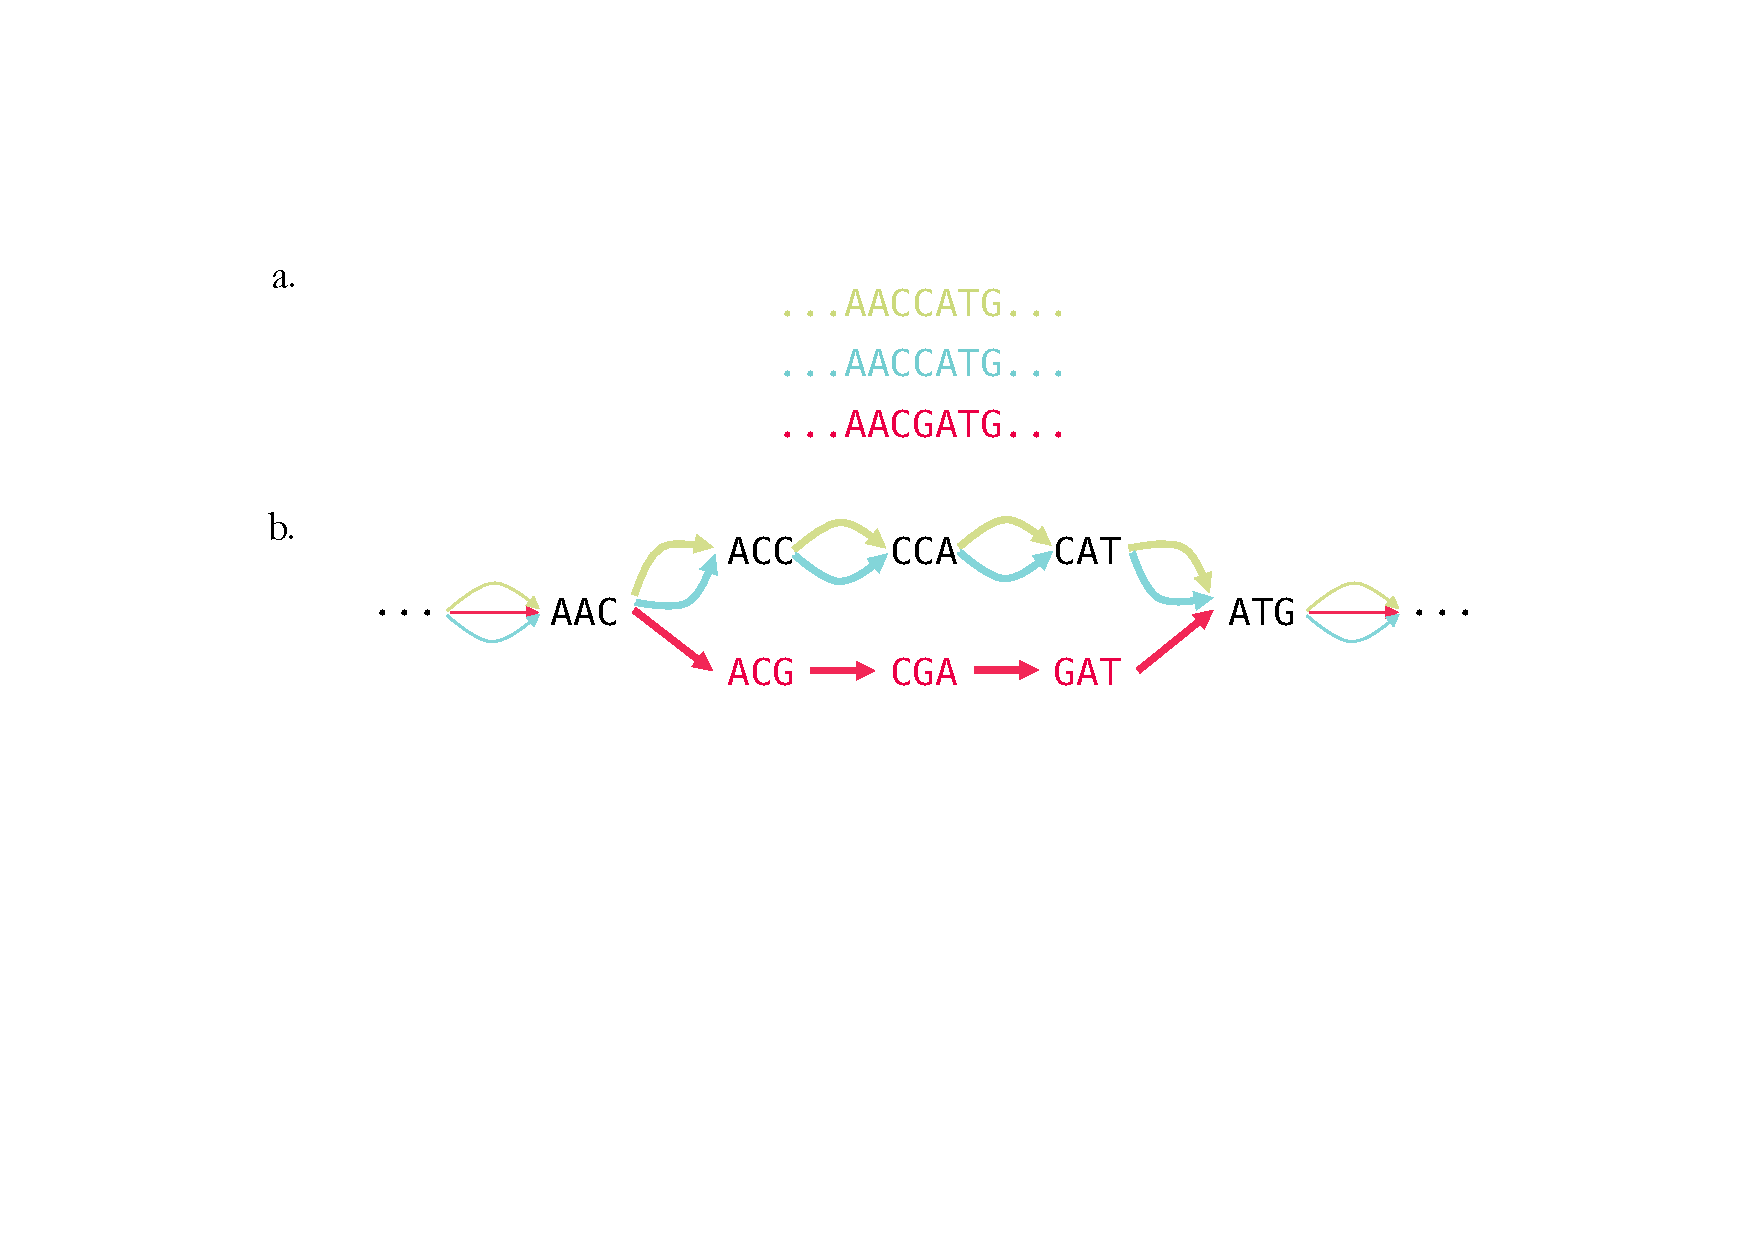
\includegraphics[width=\textwidth]{db_graph_cartoon}
  \caption{a. Haploid sequences from a mother (green), father (blue), and child (red), the last differing from the first two by a single SNP.  b. The resulting multi-color de Bruijn graph for $k=3$. Red vertices denote kmers that are deemed "novel", i.e. present in the child and absent in the parents. Edge colors reflect the samples in which the connected pairs of kmers are found. Edges that are part of the bubble (variant call) are displayed with thicker lines.}
  \label{fig:db_graph_cartoon}
\end{figure}

\begin{figure}[h!]
  \centering
    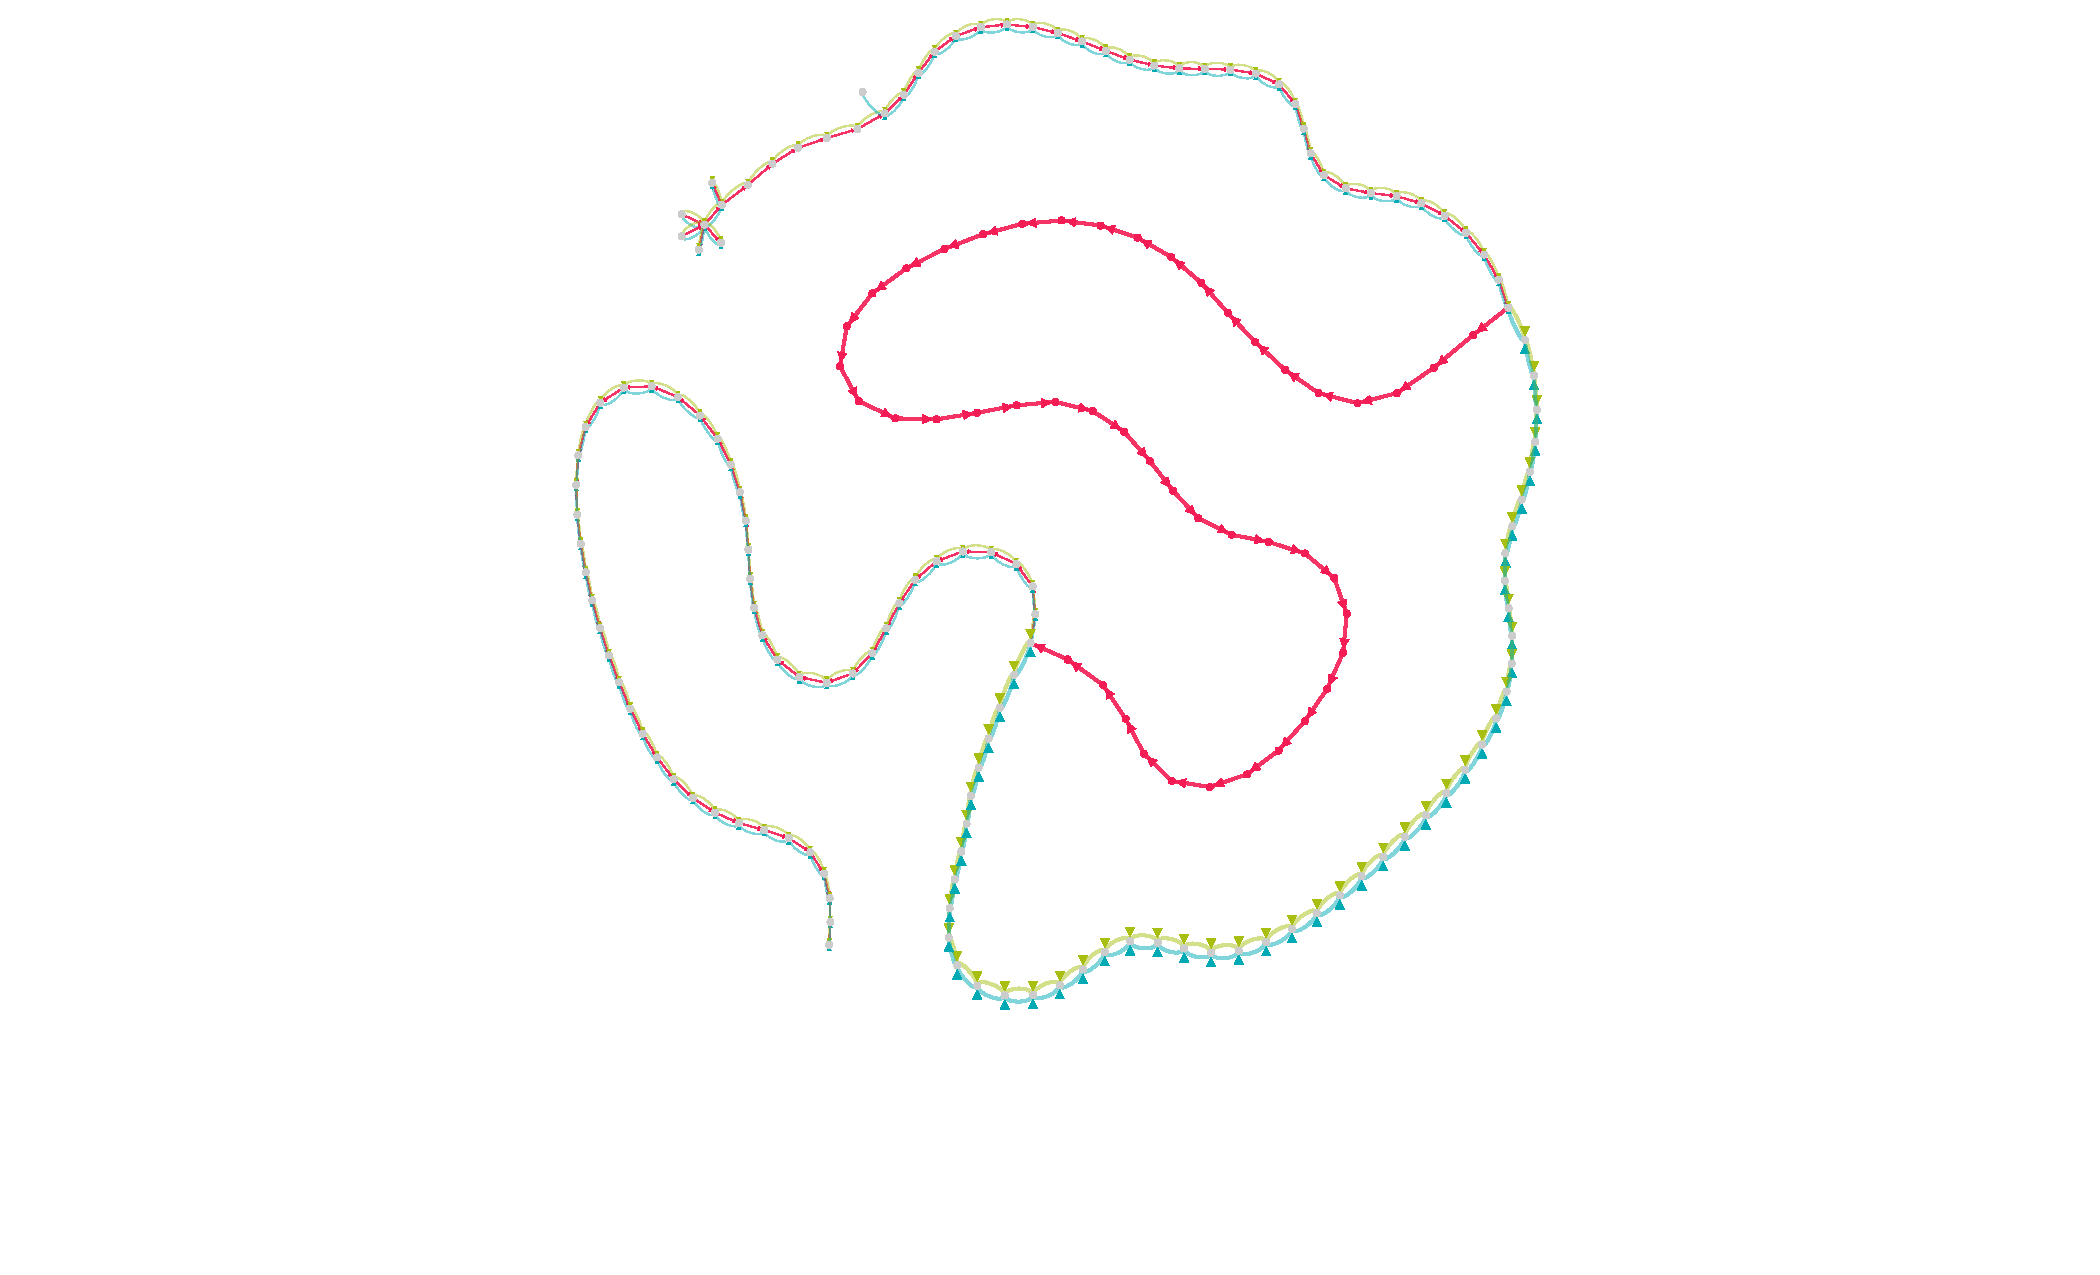
\includegraphics[width=0.5\textwidth]{snp_no_errors}
  \caption{A multi-color de Bruijn graph at $k=47$ for a haploid pedigree spanning a simulated \textit{de novo} SNP.  Vertex labels have been supressed for clarity.  Spatial layout is arbitrary and for display purposes only.}
  \label{fig:snp_no_errors}
\end{figure}

All simple variants will have this basic structure: a bubble in the graph that separates the variant samples from the non-variant samples.  The only major difference is the length of each branch: longer for an insertion in the child, shorter for a deletion (note that for short events, this is generally not apparent from the display, as evidenced by figures \ref{fig:ins_no_errors} and \ref{fig:del_no_errors}).

\begin{figure}[h!]
  \centering
    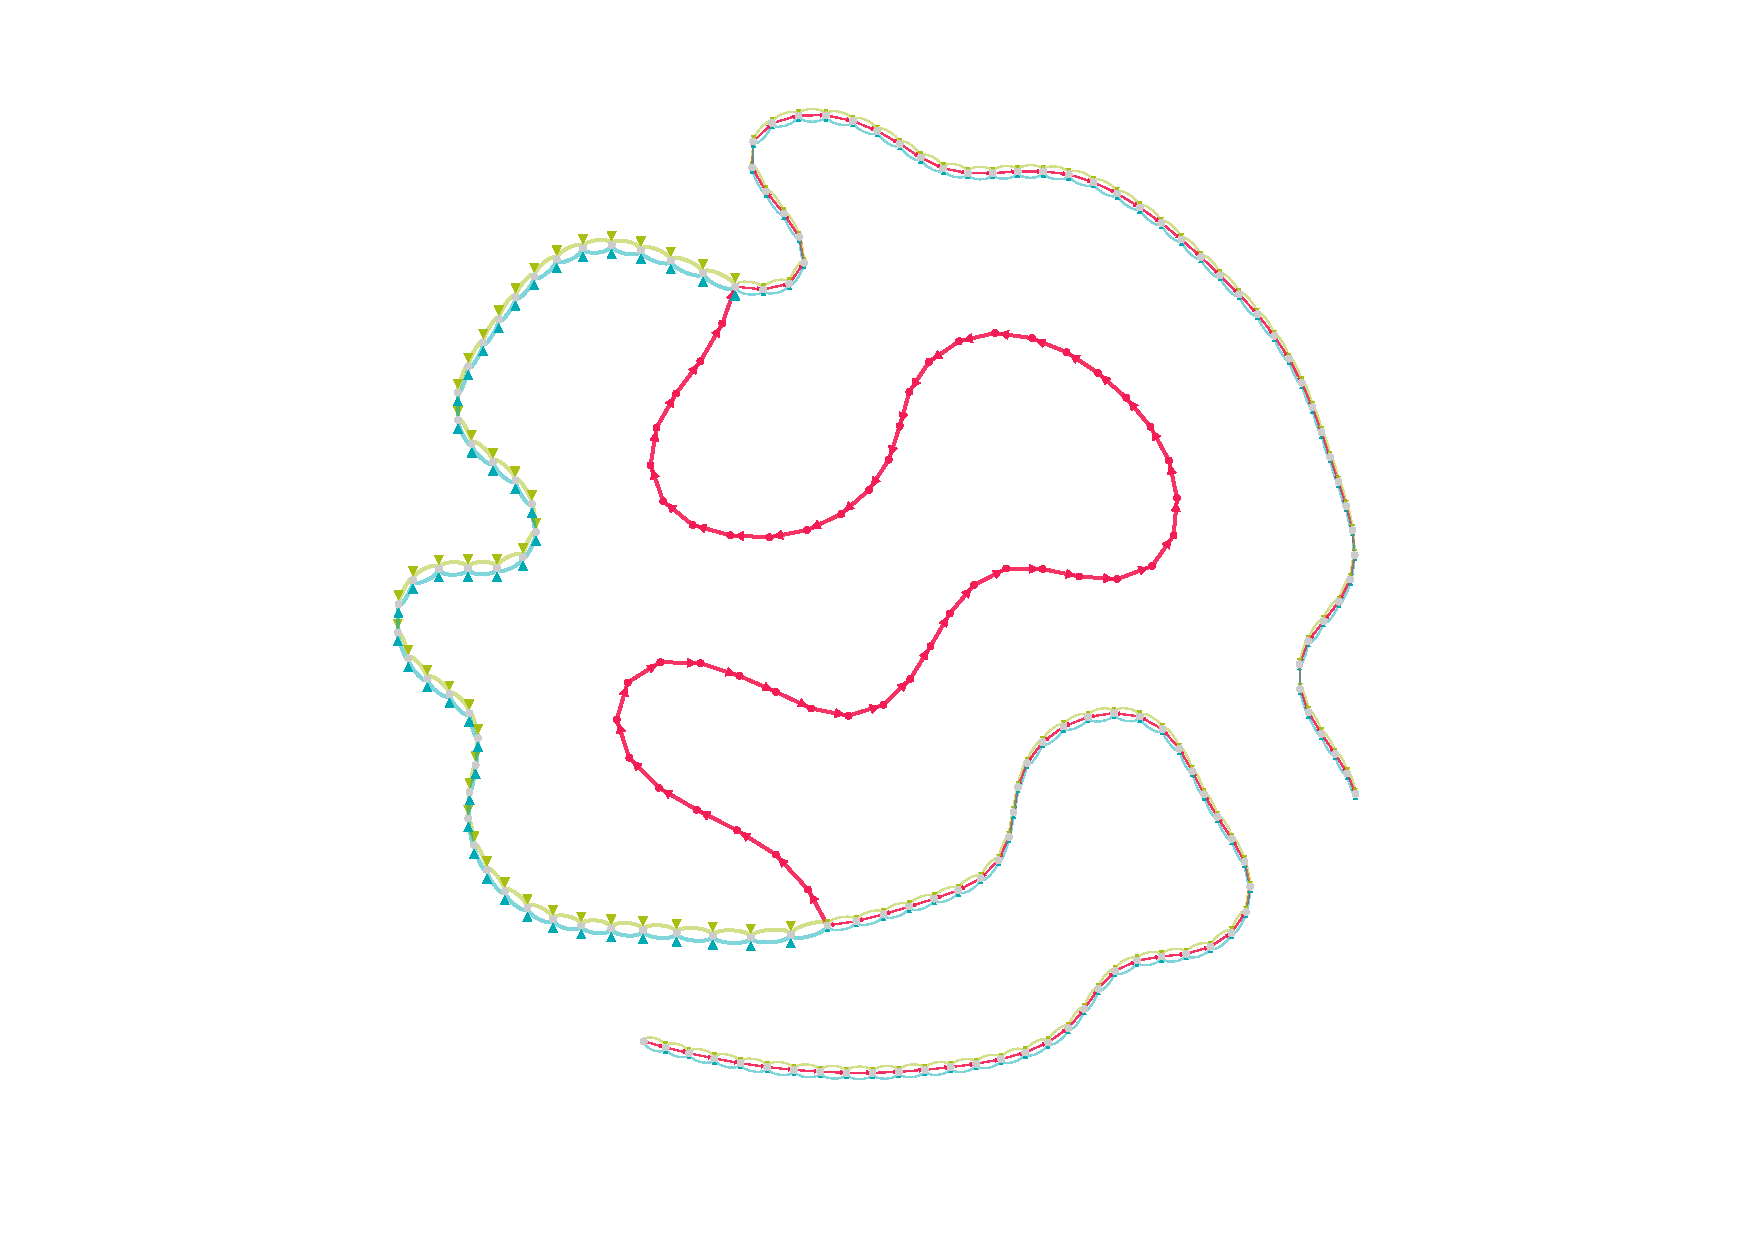
\includegraphics[width=0.5\textwidth]{ins_no_errors}
  \caption{A $5$ bp insertion in the child}
  \label{fig:ins_no_errors}
\end{figure}

\begin{figure}[h!]
  \centering
    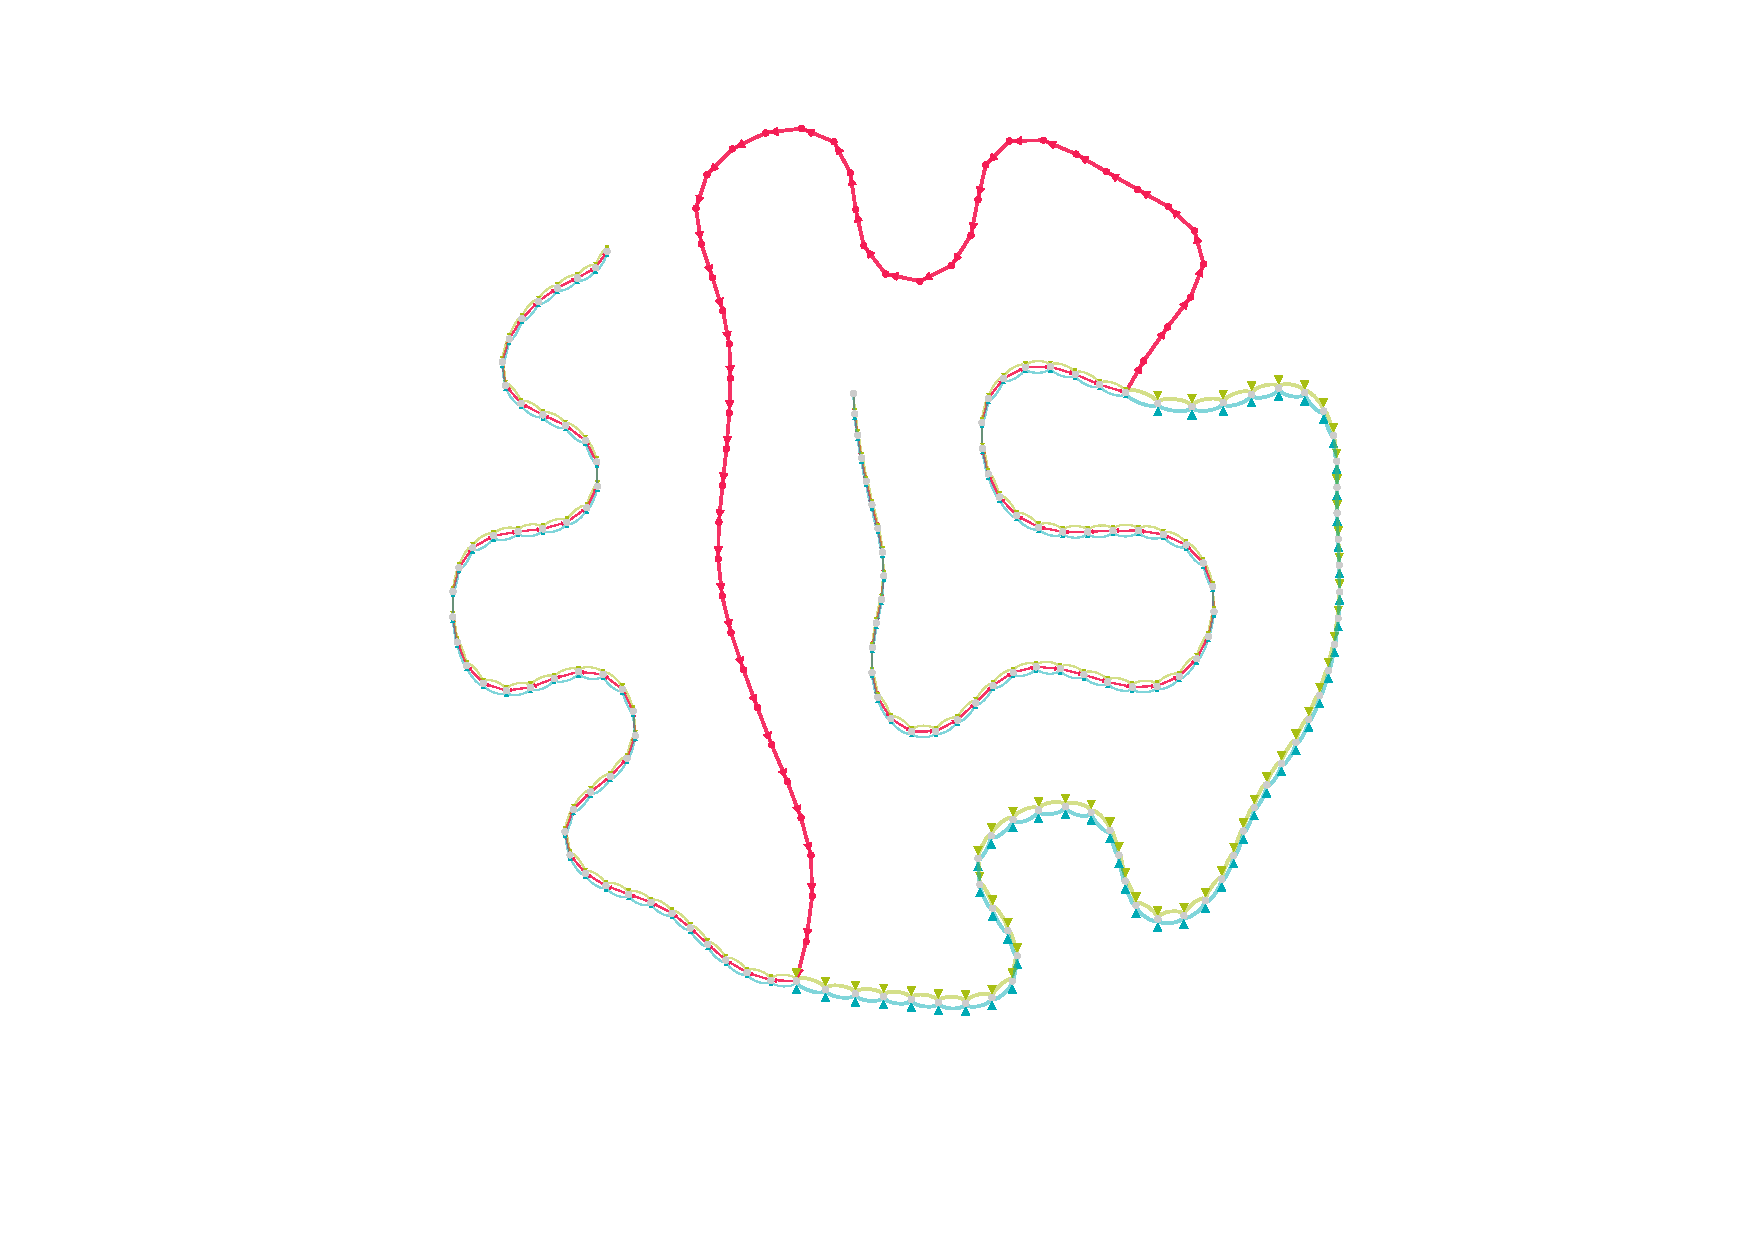
\includegraphics[width=0.5\textwidth]{del_no_errors}
  \caption{A $5$ bp deletion in the child}
  \label{fig:del_no_errors}
\end{figure}

Many variants may occur on the haplotypic background of one parent and not the other.  This is common in regions of the genome that are divergent between the two parents.  Figure \ref{fig:td_haplotypic_background} depicts one such simulated event.  A 41-bp tandem duplication has occurred on the background of the mother (evidenced by the presence of green edges), but not the father (thus the absence of blue edges).  In the flanking tails, edges shared between all three samples are present until a blue edge separates from the graph and connects to different vertices.  While not shown, these branches continue along the genome of the father.

\begin{figure}[h!]
  \centering
    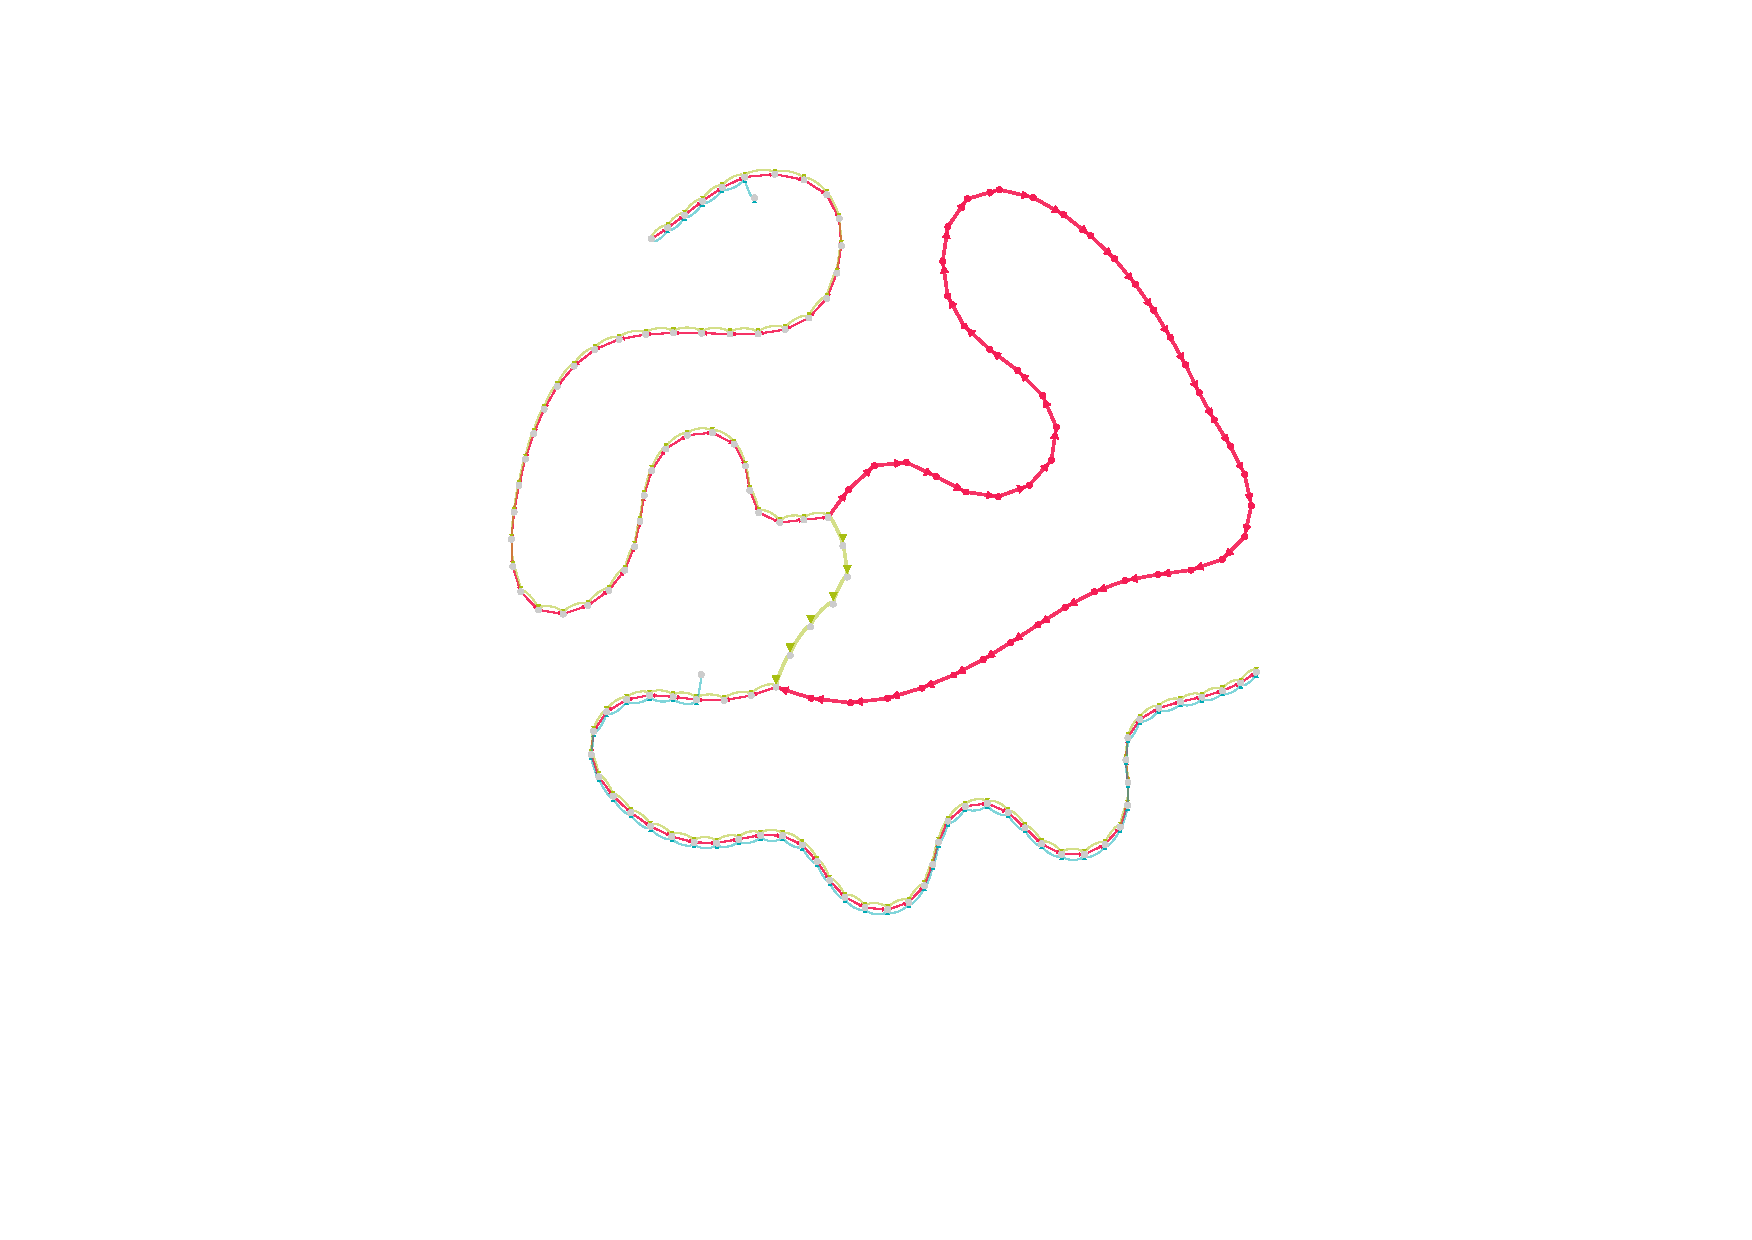
\includegraphics[width=0.5\textwidth]{td_haplotypic_background}
  \caption{A tandem duplication on the haplotypic background of the mother.}
  \label{fig:td_haplotypic_background}
\end{figure}

Finally, it is possible to encounter variants where the path through the graph taken by the child can appear to follow both the variant and non-variant paths, as demonstrated by figure \ref{fig:inv_child_follows_parents}.  Such a scenario may arise by a mutation on a sequence with copy number greater than $1$: both the unaltered and altered sequences would then exist simultaneously in the child's genome.

\begin{figure}[h!]
  \centering
    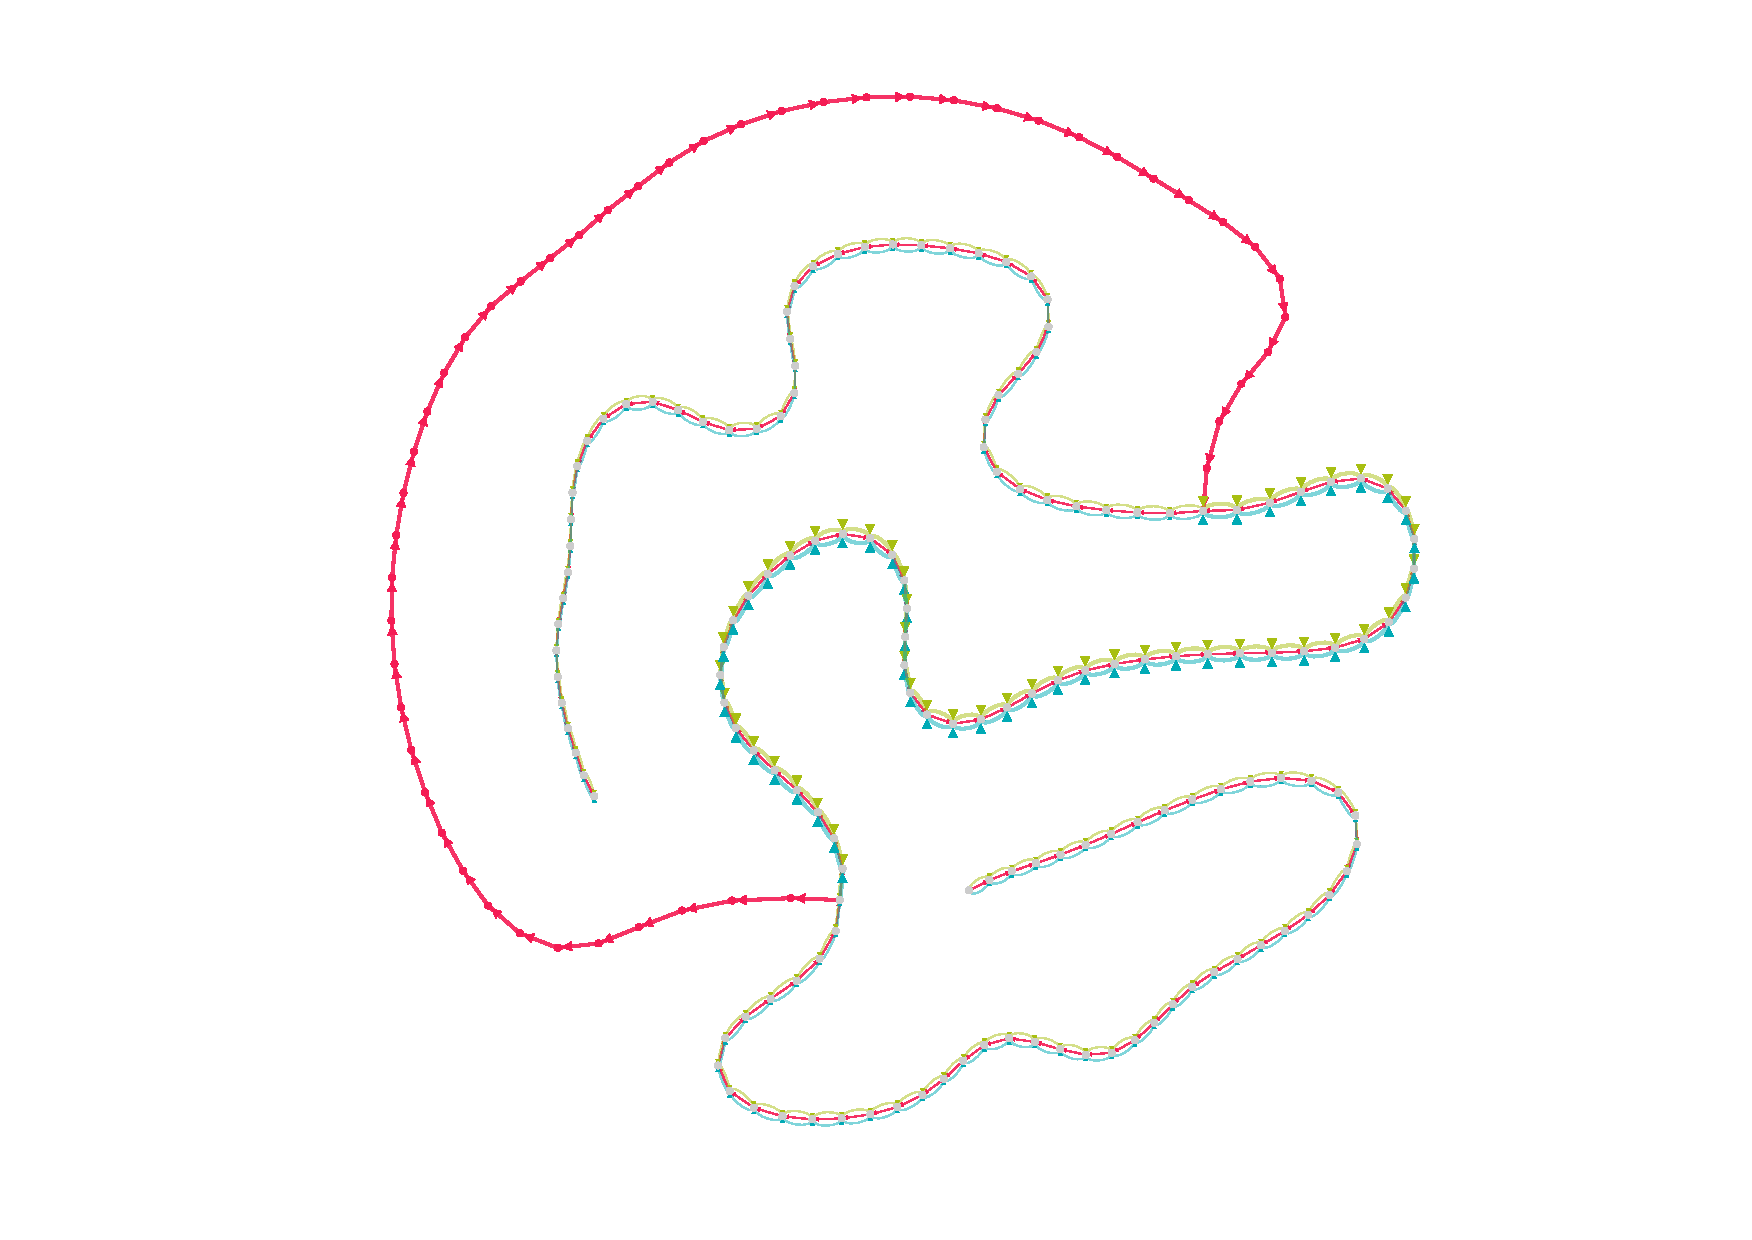
\includegraphics[width=0.5\textwidth]{inv_child_follows_parents}
  \caption{A variant wherein the child's path does not simply diverge from that of the parents, but rather navigates both.}
  \label{fig:inv_child_follows_parents}
\end{figure}

\subsection{Complex variant motifs}

Recombination events (allelic crossovers or gene conversion events; NAHR events) will not necessarily appear as bubbles.  Bubbles form in the graph when parental and progeny haplotypes diverge (at the site of a variant) and reconnect (at the flanking homologous regions).  In a recombination event, the haplotypes do not necessarily reconnect.  In a crossover or gene conversion event, as in Figure \ref{fig:recomb}, the progeny's graph should follow one parent or the other, switching at the crossover site.  Gene conversions and other multiple crossovers may switch back and forth several times.  These events can be detected simply by keeping track of which parent's graph is apparently being followed.  However, we caution the reader that it's quite likely that many events of this nature will likely go uncalled or improperly called.  For such recombination events to be detected, a kmer spanning two proximal variants must be present.  This is unlikely to occur for simple crossovers, particularly in genomes of reasonably low heterozygosity, as neighboring variants beyond a kmer's length away will not give rise to novel kmers necessary for the event's detection.  It is perhaps slightly more likely for gene conversion events, where the multiple crossovers proximal to a variant exclusive to one of the parents will generate the sought-after novel kmer signal.

NAHR events are trickier; as these events are generally mitotic rather than meiotic events, the expected motif is that a child's graph should follow the same parent, but connect disjoint components of the graph (e.g. telomeres of different chromosomes) through novel kmers.  In principle, one should be able to detect such an event by testing whether removing the child's contribution to the pedigree subgraph results in disrupting the otherwise connected components\cite{Hopcroft:1971vx}.  In practice, however, NAHR events are mediated by homology between low-complexity regions of the subtelomeric genomic regions.  The homology will result in confounding connections between disparate regions of the graph.  An easier solution is to track the parent apparently being copied from and determine the chromosome of origin for each kmer present in the flanking regions of the novel kmers.  This is only feasible if one happens to have draft reference genomes for which a kmer's chromosome of origin can be approxiately determined.

\subsection{Handling errors in sequencing}

Bubble and non-bubble motifs are trivial to find and navigate if there are no errors in the sequence data, but much more difficult to navigate in the presence of errors.  Errors manifest as extraneous branches in the graph, adding ambiguity to traversals.  Without a guide as to which branch to explore at a junction, we are either forced to abandon the traversal, make a guess, or explore all possible branches.  The former is overly conservative; many variants will go untyped.  The second is hazardous; there's the very real potential for choosing erroneously and typing the variant incorrectly.  The latter is computationally expensive; errors explore the complexity of the graph, making it very difficult (if not impossible) to find the correct path through the graph.

To solve this, recall that DNMs do more than open up a bubble motif in the graph.  Idaelly, each kmer along the variant path is novel.  If we assume that branches following the novl branch at junctions are correct and linked with the current variant being explored, we can use these novel kmers as "sign posts" to mark successful traversals.  Navigating a branch and not seeing a sign post gives us adqeuate cause to abandon a branch in favor of another.

\section{Calling and classifing \textit{de novo} variants}

Armed with an intuition as to how graphs behave in regions of \textit{de novo} variation, we can now describe the procedure for identifying and classifying a variant.  The overview involves five big steps (and associated substeps):

\begin{enumerate}
\item Identify confident and trusted novel kmers
\item Construct multi-color de Bruijn "trio" graphs (child, mother, father)
\item Load subgraph local to a novel kmer
\item Identify and classify variants in the subgraph
\item Evaluate performance
\end{enumerate}

We discuss these in details in the sections below.

\subsection{Identify confident and trusted novel kmers}

We first seek to build a list of novel kmers that are both \textit{confident} (i.e. unlikely to be sequencing errors) and \textit{trusted} (i.e. are unlikely to be the result of contamination).  Identification of the novel kmers themselves is trivial; we simply build a list of kmers that appear in the child but are completely absent in the parents.  The subsequent filtering steps are described below.

\subsubsection{Remove low coverage kmers}

For a deeply sequenced sample, we expect all kmers in the genome to be of similarly high coverage.  While there will inevitably be regions of the genome where coverage is poor owing to failure to amplify regions with high GC content, the Lander-Waterman statistics in Chapter \ref{ch:motivation} suggest we should easily see many copies of the entire \textit{P. falciparum} genome at a coverage of $100x$.  We can therefore assume that failure to reach a certain coverage threshold is indicative of sequencing error, and such kmers can be removed as candidates from the novel kmer list.

The problem remains as to where the threshold should be set.  We plotted the histogram of kmer coverage, shown in Figure \ref{fig:covthreshold}, smoothing the resulting distribution with a non-parametric LOESS fit.  The smoothed histogram makes it easier to find the first local minimum using Algorithm \ref{alg:localminimum}.

\begin{algorithm}
\caption{Compute the local minimum of a kmer coverage distribution}
\label{alg:localminimum}
\begin{algorithmic}[1]
\Function{firstLocalMinimum}{coverageHist}
    \State $y = laggedDifferences(c(INT_MAX, x)) > 0L$
    \State $y = cumSum(equalRunLengths(y).lengths)$
    \State $y = y[seq(2L, length(y), 2L)]$

    \State $\textrm{return(y[2])}$
\EndFunction
\end{algorithmic}
\end{algorithm}

\begin{figure}[h!]
  \centering
    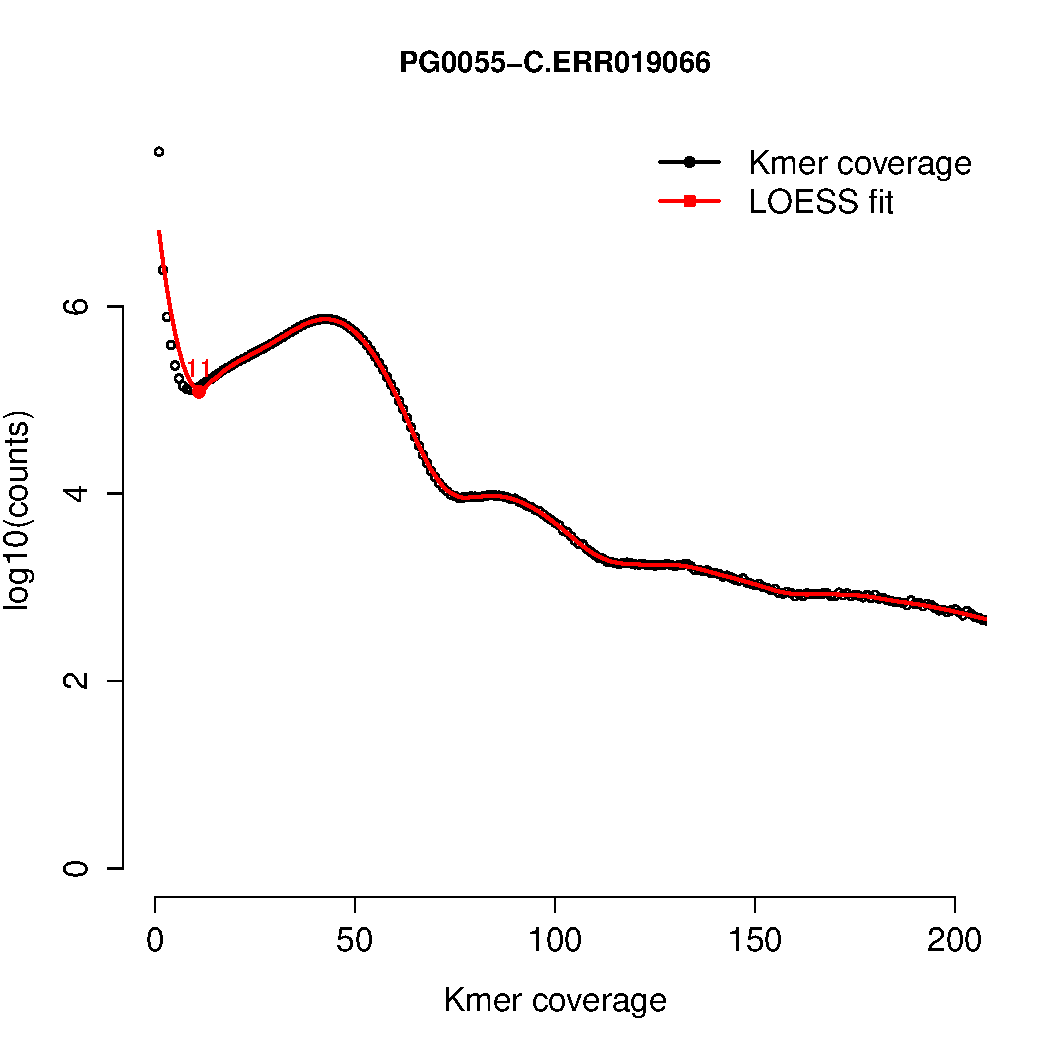
\includegraphics[width=0.9\textwidth]{covthreshold}
  \caption{Kmer coverage histogram for a real sample, with LOESS fit}
  \label{fig:covthreshold}
\end{figure}

\subsubsection{Remove possible contaminants}

Contamination can occur during sequencing library preparation due to handling from human operators (transferring either bacterial or human genetic material to the library) or from other samples (often from different species) being processed in the same laboratory.  Contamination would result in kmers that appear novel - owing to their absense in the parents - but are irrelevant for our study.  It is perhaps not a paramount concern when processing \textit{P. falciparum} data, as the genome is very different than any other sample likely to be a contaminant.  However, it may contribute a false-positive rate that we can easily mitigate.

To remove the effects of contamination, we run every confident novel kmer through BLAST\cite{Altschul:1990dw}.  Specifically, we used the \texttt{blastn} package and all available BLAST nucleotide databases to identify the likely species of every confident novel $47$-mer in each sample.  Any unidentified kmer or apparently \textit{P. falciparum} kmer was retained; all others were removed.  In practice, this removes anywhere from dozens to thousands of kmers from needing to be considered; as evidenced by Figure \ref{fig:contam}, the exact number varies as each sample is prepared independently, at different times and by different personnel.

\begin{sidewaysfigure}[h!]
  \centering
    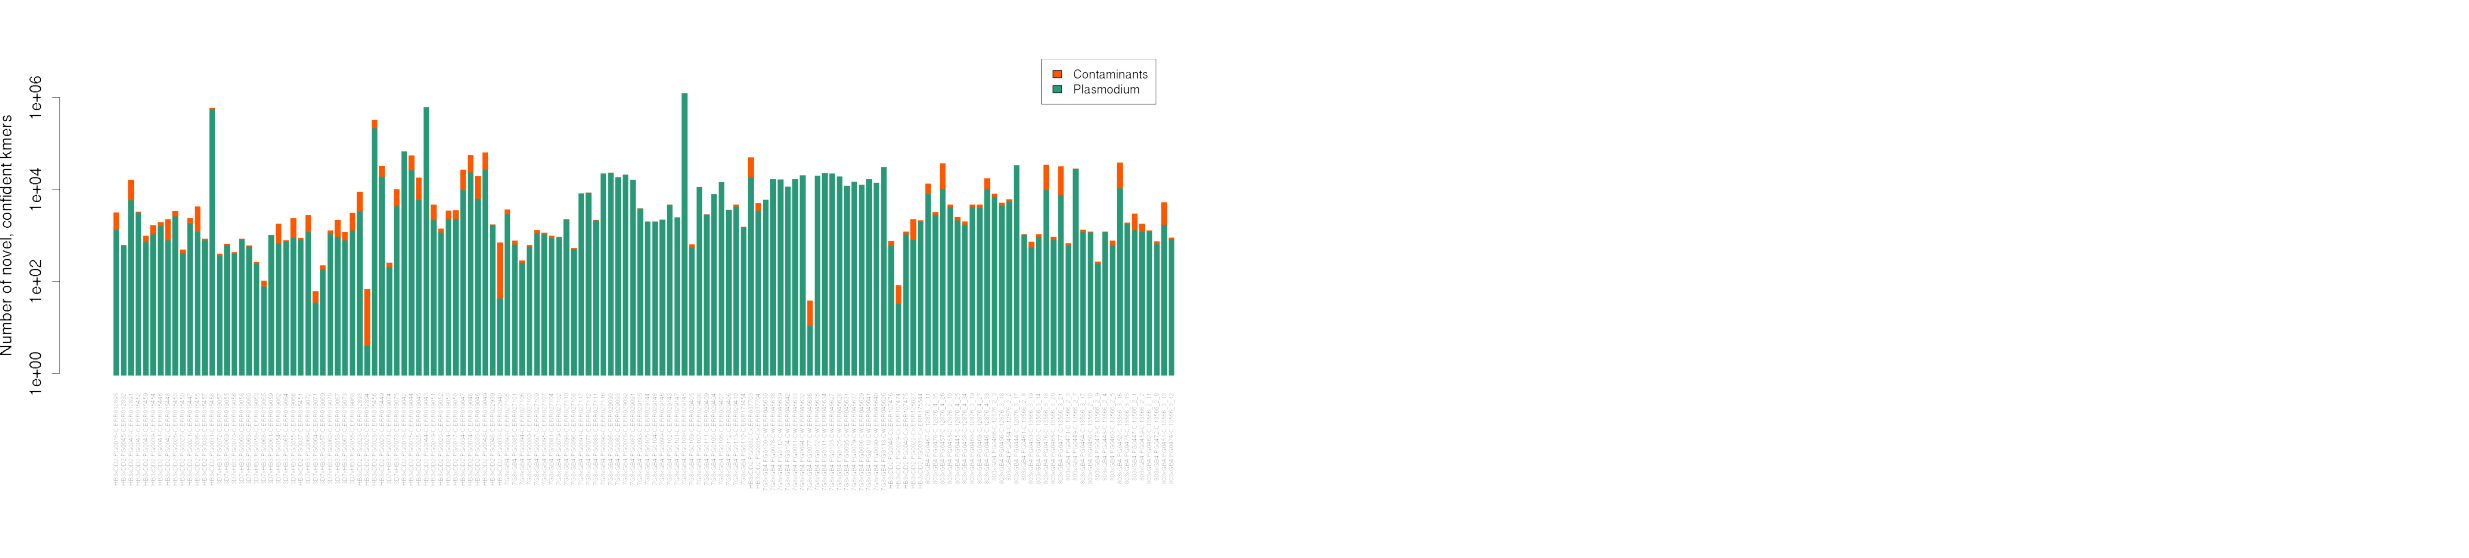
\includegraphics[width=\textwidth]{contam}
  \caption{Removal of contaminating kmers; \textit{P. falciparum} kmers are shown in green; the putative contaminants are shown in orange.}
  \label{fig:contam}
\end{sidewaysfigure}

\subsection{Construct multi-color de Bruijn "trio" graphs}

To construct the "trio" graphs, we perform assembly on each sample with the \textit{Cortex} \textit{de novo} assembly software\cite{Iqbal:2012fx} following the recommended workflow\cite{Turner:2015ve}.  Briefly, each sample is assembled using the \texttt{build} command at a kmer size of $47$ bp\footnote{This setting results from evaluations on optimal kmer size for maximizing contig length, despite not needing to produce contigs for our analyses} and ignoring nucleotides with an Illumina quality score less than $5$.  Each sample was then cleaned of likely sequencing errors with the \texttt{clean} command using automatically calculated coverage and supernode (unambiguous runs of kmers with in/out degree of $1$) length thresholds.  Finally, the graph for the child was merged into a \textit{clean} trio graph, and separately, a \textit{dirty} trio graph (one using the uncleaned graph data) using the \texttt{join} command.  This multi-color graph consists of child, mother, and father.  For our purposes with \textit{P. falciparum}, "child" is assigned color $0$, "mother" (the first parent of the cross) to color $1$, and "father" to color $2$.  Read threading was \textit{not} applied, as in our analyses, there is no need for contigs, just the graph data structure.

\subsection{Load subgraph local to a novel kmer}

To facilitate variant calling, we must process regions of the graph likely to harbor DNMs.  While it is technically possible to load a \textit{P. falciparum} graph into RAM (owing to its small $23$ megabase genome), it is unlikely such a solution would scale to larger genomes.  It is also cumbersome to do so when there are only on the order of dozens, perhaps hundreds, of variants to be discovered per genome.  Therefore, we adopted a solution of fetching only relevant parts of the genome as necessary, operating on the local subgraph surrounding the putative variant, rather than on the entire graph at once.

\subsubsection{Depth-first search}

Graph exploration is an \textit{online} problem, meaning the structure of the graph cannot be known until it is explored.  As a non-linear data structure, it is not trivial to determine where to start and stop exploring a graph.  During traversal, one may encounter junctions (due to errors or homology) without any additional information as to which branch to choose.  Graphs sometimes loop back onto themselves, necessitating that we keep track of our walk so that we do not end up traversing endlessly in circles.  Incorrect decisions in the traversal cannot always be detected, requiring appropriate stopping conditions to abort a traversal if no fruitful data is discovered.

Typically, graph exploration can be accomplished with a so-called \textit{depth-first search}, or DFS.  The basic premise of a DFS is summarized in Algorithm \ref{alg:dfs}: start at a vertex, walk in a chosen direction until a junction is encountered, choose one branch and repeat the DFS from that point until it is deemed appropriate to stop, then jump back to the junction to choose the next branch, and repeat until completion.  In practice, this approach has some drawbacks that manifest quickly in real data.  First, the basic DFS algorithm terminates only when there are no more vertices left to traverse, which is overkill for our purposes.  Second, all branches are treated equally.  For our purposes, branches containing errors are not important and should be discarded lest they confuse later algorithms trying to find paths through bubbles in order to type variants.  Third, this requires us to explore three graphs separately, which is inefficient.

\begin{algorithm}
\caption{A basic, iterative depth-first search}
\label{alg:dfs}
\begin{algorithmic}[1]
\Function{idfs}{graph, vertex}
  \State $s = \textrm{new Stack()}$
  \State $\textrm{visited} = \{\}$
  \State $\textrm{s.push(vertex)}$

  \While{\textrm{!s.isEmpty()}}
    \State $current = s.pop()$
    \If{$\textrm{visited.contains(current)}$}
        \State $\textrm{next}$
    \EndIf
    \State $\textrm{visited.add(current)}$

    \For{$\textrm{v in graph.nextVertices(vertex)}$}
        \State $\textrm{s.push(v)}$
    \EndFor
  \EndWhile
\EndFunction
\end{algorithmic}
\end{algorithm}

The solution is to instead conduct a DFS with stopping conditions and recursively.  Stopping conditions, specifying the conditions upon which a traversal is deemed "successful" or "failed" allow us to decide certain branches in the subgraph are unfruitful for analysis.  The recursive traversal allows us to act on the result of the stopping condition, adding it to the subgraph if successful, discarding it if not.  This is described in Algorithm \ref{alg:rdfs}.

\begin{algorithm}
\caption{The recursive depth-first search with arbitrary stopping conditions}
\label{alg:rdfs}
\begin{algorithmic}[1]
\Function{rdfs}{clean, dirty, kmer, color, g, stopper, depth, goForward, history}
    \State firstKmer = kmer

    \State sourceKmersAllColors = goForward ? getPrevKmers(clean, dirty, kmer) : getNextKmers(clean, dirty, kmer)
    \State sourceKmers = sourceKmersAllColors.get(color)

    \State dfs = new Graph<AnnotatedVertex, AnnotatedEdge>()
    \State stopper = instantiateStopper(stopperClass)

    \Repeat
        \State cv = kmer

        \State cr = clean.findRecord(cv)
        \If{(cr == null \&\& dirty != null)}
            \State cr = dirty.findRecord(cv)
        \EndIf

        \State prevKmers = CortexUtils.getPrevKmers(clean, dirty, cv);
        \State nextKmers = CortexUtils.getNextKmers(clean, dirty, cv));
        \State adjKmers  = goForward ? nextKmers : prevKmers;

        \State numVerticesAdded = addVertexAndConnect(dfs, cv, prevKmers, nextKmers)

        \If{stopper.keepGoing(cr, g, depth, dfs.vertexSet().size(), adjKmers.get(color).size()) \&\& !sourceKmers.contains(kmer) \&\& !history.contains(kmer)}
            \State history.add(kmer);

            \If{adjKmers.get(color).size() == 1}
                \State kmer = adjKmers.get(color).iterator().next();
            \ElsIf{adjKmers.get(color).size() != 1}
                \State childrenWereSuccessful = false;

                \For{ak in adjKmers.get(color)}
                    \If{(!ak.equals(firstKmer))}
                        \State branch = dfs(clean, dirty, ak, color, g, stopperClass, depth + isNovelKmer(cr) ? 0 : 1, goForward, history)

                        \If{branch != null}
                            \State Graphs.addGraph(dfs, branch)
                            \State childrenWereSuccessful = true
                        \Else
                            \For{av in dfs.vertexSet()}
                                \If{av.getKmer().equals(ak)}
                                    \State av.setFlag("branchRejected")
                                \EndIf
                            \EndFor
                        \EndIf
                    \EndIf
                \EndFor

                \If{childrenWereSuccessful || stopper.hasTraversalSucceeded(cr, g, depth, dfs.vertexSet().size(), 0)}
                    \State return dfs
                \Else
                    \For{av in dfs.vertexSet()}
                        \If{(av.getKmer().equals(kmer))}
                            \State av.setFlag("branchRejected")
                        \EndIf
                    \EndFor
                \EndIf
            \EndIf
        \ElsIf{stopper.traversalSucceeded()}
            \State return dfs
        \Else
            \State return null
        \EndIf
    \Until{(adjKmers.get(color).size() == 1)}

    \State return null
\EndFunction
\end{algorithmic}
\end{algorithm}

Stopping conditions are implemented as a callback object, permitting programmer-specified limits for different situations.  To type DNMs, we begin traversal at a novel kmer, walking forward and backward in the graph until the stopping conditions are met.  We then explore the parental graphs based on the subgraph we loaded for the child.  As the parental traversals have some additional information (namely, the presence of the child's subgraph allows us to check if a parental traversal has diverged and rejoined from the graph), the stopping conditions are different.

The stopping condition callback object implements two boolean methods: \texttt{hasTraversalSucceeded} and \texttt{hasTraversalFailed}.  Both of them may return \texttt{false}, in which case the traversal continues.  If either returns \texttt{true}, traversal is halted and the branch is evaluated for retention or rejection.

\subsubsection{Stopping conditions for child}

The child's stopping conditions on traversal success or failure are provided in Algorithm \ref{alg:child_hasTraversalSucceded} and \ref{alg:child_hasTraversalFailed}, respectively.  For the child, success is approximately determined by having explored a novel kmer stretch in the graph to the point that it has rejoined the parental graphs.  However, we purposefully continue reading another $50$ kmers before returning success.  If more novel kmers are recovered in that span, we reset our counters and continue walking.  This facilitates two things: the absence of novel kmers due to sequencing errors or overthresholding, and typing complex variants that may have short stretches of non-novel kmers.  Failure is determined by a number of criteria, including the absence of novel kmers, low complexity regions, having no more branches to explore, having reached a maximum graph depth, or having reached a maximum graph size.

\begin{algorithm}
\caption{Child's traversal success determination method}
\label{alg:child_hasTraversalSucceded}
\begin{algorithmic}[1]
\Function{hasTraversalSucceeded}{cr, g, depth, size, edges}
    \If{goalSize == 0 \&\& (cr.getCoverage(1) > 0 || cr.getCoverage(2) > 0)}
        \State goalSize = size
        \State goalDepth = depth
    \EndIf

    \If{goalSize > 0 \&\& isNovel(cr)}
        \State goalSize = size
        \State goalDepth = depth
    \EndIf

    \State return (goalSize > 0 \&\& (size >= goalSize + 50 || isLowComplexity(cr) || edges == 0))
\EndFunction
\end{algorithmic}
\end{algorithm}

\begin{algorithm}
\caption{Child's traversal failure determination method}
\label{alg:child_hasTraversalFailed}
\begin{algorithmic}[1]
\Function{hasTraversalFailed}{cr, g, depth, size, edges}
    \State return !isNovel(cr) \&\& (isLowComplexity(cr) || edges == 0 || depth >= 5 || size > 5000)
\EndFunction
\end{algorithmic}
\end{algorithm}

\subsubsection{Stopping conditions for parents}

The parents' stopping conditions on traversal success or failure are provided in Algorithm \ref{alg:parent_hasTraversalSucceded} and \ref{alg:parent_hasTraversalFailed}, respectively.  Success is determined by having diverged from the child's graph and rejoined it.  Care is taken to ensure that we have rejoined the graph at a boundary of the novel kmer stretch, rather than some ther part of the graph obtained when trying to read some extra flanking data in Algorithm \ref{alg:child_hasTraversalSucceded}.  Failure is determined by a number of criteria, including having reached a maximum graph size, having reached a maximum graph depth, or low complexity regions.

\begin{algorithm}
\caption{Parents' traversal success determination method}
\label{alg:parent_hasTraversalSucceded}
\begin{algorithmic}[1]
\Function{hasTraversalSucceeded}{cr, g, depth, size, edges}
    \State fw = cr.getKmerAsString()
    \State rc = reverseComplement(fw)
    \State v = null
    \State rejoinedGraph = false

    \If{ g.containsVertex(fw) || g.containsVertex(rc) }
        \State rejoinedGraph = true

        \For{av in g.vertexSet()}
            \If{ (av.getKmer().equals(fw) || av.getKmer().equals(rc)) }
                \If{ (!sawPredecessorFirst \&\& !sawSuccessorFirst) }
                    \If{ (av.flagIsSet("predecessor")) }
                        sawPredecessorFirst = true 
                    \ElsIf{ (av.flagIsSet("successor")) }
                        sawSuccessorFirst = true 
                    \EndIf
                \EndIf

                \If{ ((sawPredecessorFirst \&\& av.flagIsSet("predecessor")) || (sawSuccessorFirst \&\& av.flagIsSet("successor"))) }
                    \State rejoinedGraph = false
                    \State break
                \EndIf
            \EndIf
        \EndFor
    \EndIf

    \State return size > 1 \&\& rejoinedGraph
\EndFunction
\end{algorithmic}
\end{algorithm}

\begin{algorithm}
\caption{Parents' traversal failure determination method}
\label{alg:parent_hasTraversalFailed}
\begin{algorithmic}[1]
\Function{hasTraversalFailed}{cr, g, depth, size, edges}
    \State return size > 1000 || junctions >= 5 || isLowComplexity(cr)
\EndFunction
\end{algorithmic}
\end{algorithm}

\subsection{Identify and classify variants in the subgraph}

With the relevant subgraph now loaded, we can now attempt to type variants.  Typing involves three steps:

\begin{enumerate}
\item Annotate vertices in the graph that can be possible start and end points of the variant bubble
\item Find the shortest path from start to end that satisfies some conditions
\item From the haplotypes, remove the flanking homologous sequence to reveal the variant alleles
\end{enumerate}

Let us first detail how we annotate the viable starts and ends of the variant, which simply amounts to iterating through each vertex in the subgraph and checking that it means various conditions.  A variant start (end) vertex should have out degree (in degree) greater than $1$.  The branches should be color-specific to reflect the opening of a bubble between the different samples in the graph.  This is detailed in Algorithm \ref{alg:annotate_subgraph}.

\begin{algorithm}
\caption{Annotating possible variant starts and ends of the subgraph}
\label{alg:annotate_subgraph}
\begin{algorithmic}
\Function{annotateStartsAndEnds}{b}
    \For{av in b.vertexSet()}
        \If{b.outDegreeOf(av) > 1}
            \State aes = b.outgoingEdgesOf(av)

            \State childEdges = \{\}
            \State parentEdges = \{\}

            \For{AnnotatedEdge ae in aes}
                \If{ae.isPresent(0) \&\& ae.isAbsent(1) \&\& ae.isAbsent(2)} 
                    \State childEdges.add(ae)
                \EndIf

                \If{ae.isPresent(color)}
                    \State parentEdges.add(ae)
                \EndIf
            \EndFor

            \If{childEdges.size() > 0 \&\& parentEdges.size() > 0 || beAggressive}
                \State av.setFlag("start")
                \State candidateStarts.add(av)
            \EndIf
        \EndIf

        \If{b.inDegreeOf(av) > 1}
            \State aes = b.incomingEdgesOf(av)

            \State childEdges = \{\}
            \State parentEdges = \{\}

            \For{AnnotatedEdge ae in aes}
                \If{ae.isPresent(0) \&\& ae.isAbsent(1) \&\& ae.isAbsent(2)}
                    \State childEdges.add(ae)
                \EndIf

                \If{ae.isPresent(color)}
                    \State parentEdges.add(ae)
                \EndIf
            \EndFor

            \If{(childEdges.size() > 0 \&\& parentEdges.size() > 0) || beAggressive} 
                \State av.setFlag("end")

                \State candidateEnds.add(av)
            \EndIf
        \EndIf
    \EndFor
\EndFunction
\end{algorithmic}
\end{algorithm}

\subsubsection{Dijkstra's shortest path algorithm}

With all of the start and end points now annotated, we now need to find a path from one end of the putative variant to the other.  The number of possible paths could be very large.  We shall make the assumption that the correct path is the shortest path.  While this will often be the case, we note that the shortest path is not necessarily the biological path.  This could be the case in highly repetitive regions longer than a kmer length.  Since de Bruijn graphs tend to collapse long repeats, we may miss some events.

E. W. Dijkstra described his shortest path algorithm in 1959\cite{Dijkstra:1959cw}.  We describe it below in Algorithm \ref{alg:dijkstra}.  Briefly, we keep track of all vertices' distance from the source vertex, setting the source's distance to itself to $0$ and all others to infinity (to denote as-of-yet unvisited vertices).  We then select the vertex with the minimum distance to the source (in the first iteration, the source itself) and compute a new distance to all immediately adjacent vertices.  This new distance is a sum of the distance traversed so far from the source to one of these vertices.  For our purposes, we shall assume the distance between two adjacent vertices is always $1$.  If the distance computed is less than the distance recorded, we replace the old value with the new.  We remove this vertex from the processing queue and proceed to the next vertex with the lowest distance from the source.

\begin{algorithm}
\caption{Finding the shortest path in a graph}
\label{alg:dijkstra}
\begin{algorithmic}
\Function{dspa}{graph, source, destination, color}
    \State dist = \{\}
    \State prev = \{\}
    \State q = []

    \ForAll{v in g.vertexSet()}
        \State dist[v] = infinity
        \State prev[v] = null
        \State push(q, v)
    \EndFor

    \State dist[source] = 1

    \While{!q.isEmpty()}
        \State u = vertexWithMinDistance(q, dist)

        \If{u == destination}
            \State break
        \EndIf

        \State q.remove(u);

        \If{u != -1}
            \ForAll{e in g.outgoingEdgesOf(u, color)}
                \State v = g.getEdgeTarget(e, color)

                \State alt = dist[u] + 1

                \If{alt < dist[v]}
                    \State dist[v] = alt
                    \State prev[v] = u
                \EndIf
            \EndFor
        \EndIf
    \EndWhile

    \State s = []
    \State Integer u = destination

    \While{u != null \&\& prev.containsKey(u)}
        \State push(s, u)
        \State u = prev[u]
    \EndWhile

    \State return s
\EndFunction
\end{algorithmic}
\end{algorithm}

To use this algorithm for allele identification, we iterate through all possible combinations of start and stop vertices, obtained as described in the previous section.  We then iterate through the three graph colors (representing the child, mother, and father).  For each color, we apply Algorithm \ref{alg:dijkstra}.  For the child, we place the additional constraint that the path accepted must contain at least one novel kmer.

This algorithm will return the child and parental haplotypes.  To identify the precise alleles of the event, we simply trim back the homologous regions of the haplotypes with Algorithm \ref{alg:trim}.

\begin{algorithm}
\caption{Finding the shortest path in a graph}
\label{alg:trim}
\begin{algorithmic}
\Function{trimHaplotypes}{child, parent}
    \State e0 = child.length() - 1
    \State e1 = parent.length() - 1
    \State s = 0
    \State length = (child.length() < parent.length() ? child.length() : parent.length())

    \For{(s = 0; s < length \&\& child[s] == parent[s]; s++)}
        \State (do nothing)
    \EndFor

    \While{(e0 > s \&\& e1 > s \&\& child[e0] == parent[e1])}
        \State e0--
        \State e1--
    \EndWhile
\EndFunction
\end{algorithmic}
\end{algorithm}

\subsubsection{Classify event}

For simple variants (those that conform to the bubble motif), event classification is reasonably straightforward.  We simply inspect the recovered alleles and evaluate them against simple rules.  For example, a SNP should be a single nucleotide in length.  An insertion should have a parental allele length of $1$ and a child allele length $> 1$.

To classify complex variants, we rely on other heuristics.  GC events are classified by keeping track of which parent the child's genome appears to be exclusively copying from (simply by measuring when kmer coverage has dropped from one parent and returned in the other), detailed in Algorithm \ref{alg:hasSwitches}.

\begin{algorithm}
\caption{Stretch has switches}
\label{alg:hasSwitches}
\begin{algorithmic}
\Function{hasSwitches}{graph, stretch}
    \State inherit = []
    \ForAll{$47$-bp kmers $k$ in stretch}
        \State cov0 = graph.getCoverage(k, 0) \Comment child
        \State cov1 = graph.getCoverage(k, 1) \Comment mother
        \State cov2 = graph.getCoverage(k, 2) \Comment father

        \If{(cov0 > 0 \&\& cov1 == 0 \&\& cov2 == 0)}
            \State append(inherit, "C")
        \ElsIf{(cov0 > 0 \&\& cov1 > 0 \&\& cov2 == 0)}
            \State append(inherit, "M")
        \ElsIf{(cov0 > 0 \&\& cov1 == 0 \&\& cov2 > 0)}
            \State append(inherit, "D")
        \ElsIf{(cov0 > 0 \&\& cov1 > 0 \&\& cov2 > 0)}
            \State append(inherit, "B")
        \EndIf
    \EndFor

    \For{i in inherit.length()}
        \For{inherit[i] == 'B'}
            \State prevContext = '?'
            \State nextContext = '?'

            \For{(j = i - 1; j >= 0; j--)}
                \If{(inherit[j] == 'M' || inherit[j] == 'D')}
                    \State prevContext = inherit[j]
                    \State break
                \EndIf
            \EndFor

            \For{(j = i + 1; j < inherit.length(); j++)}
                \If{(inherit[j] == 'M' || inherit[j] == 'D')}
                    \State nextContext = inherit[j];
                    \State break;
                \EndIf
            \EndFor

            \State context = '?';
            \If{(prevContext == nextContext \&\& prevContext != '?')}
                \State context = prevContext
            \ElsIf{(prevContext != nextContext)}
                \If{(prevContext != '?')}
                    \State context = prevContext
                \Else
                    \State context = nextContext
                \EndIf
            \EndIf

            \State inherit[i] = context
        \EndFor
    \EndFor

    \State return inheritStr.matches(".*D+.C+.M+.*") || inheritStr.matches(".*M+.C+.D+.*")
\EndFunction
\end{algorithmic}
\end{algorithm}

\subsubsection{Mark traversed novel kmers as used}

\subsection{Evaluate performance}
\subsubsection{Generate novel kmer to variant map}
\subsubsection{Load variant containing a novel kmer}
\subsubsection{Compare alleles}

\subsection{Summary}

\section{Results on simulated data}

\begin{table}[]
\centering
\caption{ROC metrics on simulated perfect data}
\label{tbl:roc_perfect}
\begin{tabular}{rlrrrrrrrrrrrrr}
\toprule
sn & sim & fp & fn & tp & tn & rc & sens & spec & prec & npv & fpr & fnr & fdr & acc\\
\midrule
5 & perfect & 1 & 5 & 126 & 22240910 & 9 & 0.9618 & 1 & 0.9921 & 1 & 0 & 0.0382 & 0.0079 & 1\\
3 & perfect & 2 & 3 & 154 & 22200660 & 4 & 0.9809 & 1 & 0.9872 & 1 & 0 & 0.0191 & 0.0128 & 1\\
0 & perfect & 0 & 2 & 106 & 22241343 & 7 & 0.9815 & 1 & 1.0000 & 1 & 0 & 0.0185 & 0.0000 & 1\\
12 & perfect & 0 & 2 & 113 & 22233659 & 3 & 0.9826 & 1 & 1.0000 & 1 & 0 & 0.0174 & 0.0000 & 1\\
13 & perfect & 0 & 2 & 114 & 22217297 & 5 & 0.9828 & 1 & 1.0000 & 1 & 0 & 0.0172 & 0.0000 & 1\\
17 & perfect & 0 & 2 & 117 & 22242890 & 6 & 0.9832 & 1 & 1.0000 & 1 & 0 & 0.0168 & 0.0000 & 1\\
1 & perfect & 1 & 2 & 137 & 22249556 & 8 & 0.9856 & 1 & 0.9928 & 1 & 0 & 0.0144 & 0.0072 & 1\\
14 & perfect & 2 & 2 & 162 & 22196410 & 7 & 0.9878 & 1 & 0.9878 & 1 & 0 & 0.0122 & 0.0122 & 1\\
11 & perfect & 1 & 1 & 114 & 22207761 & 2 & 0.9913 & 1 & 0.9913 & 1 & 0 & 0.0087 & 0.0087 & 1\\
6 & perfect & 1 & 1 & 118 & 22203683 & 2 & 0.9916 & 1 & 0.9916 & 1 & 0 & 0.0084 & 0.0084 & 1\\
8 & perfect & 1 & 1 & 129 & 22229379 & 5 & 0.9923 & 1 & 0.9923 & 1 & 0 & 0.0077 & 0.0077 & 1\\
10 & perfect & 0 & 1 & 130 & 22238480 & 2 & 0.9924 & 1 & 1.0000 & 1 & 0 & 0.0076 & 0.0000 & 1\\
15 & perfect & 1 & 1 & 131 & 22208991 & 10 & 0.9924 & 1 & 0.9924 & 1 & 0 & 0.0076 & 0.0076 & 1\\
16 & perfect & 1 & 1 & 166 & 22213928 & 4 & 0.9940 & 1 & 0.9940 & 1 & 0 & 0.0060 & 0.0060 & 1\\
2 & perfect & 1 & 0 & 105 & 22225262 & 3 & 1.0000 & 1 & 0.9906 & 1 & 0 & 0.0000 & 0.0094 & 1\\
4 & perfect & 2 & 0 & 72 & 22210167 & 2 & 1.0000 & 1 & 0.9730 & 1 & 0 & 0.0000 & 0.0270 & 1\\
7 & perfect & 1 & 0 & 57 & 22225612 & 1 & 1.0000 & 1 & 0.9828 & 1 & 0 & 0.0000 & 0.0172 & 1\\
9 & perfect & 0 & 0 & 107 & 22255460 & 2 & 1.0000 & 1 & 1.0000 & 1 & 0 & 0.0000 & 0.0000 & 1\\
18 & perfect & 2 & 0 & 133 & 22242522 & 0 & 1.0000 & 1 & 0.9852 & 1 & 0 & 0.0000 & 0.0148 & 1\\
19 & perfect & 1 & 0 & 98 & 22236313 & 6 & 1.0000 & 1 & 0.9899 & 1 & 0 & 0.0000 & 0.0101 & 1\\
\bottomrule
\end{tabular}
\end{table}

\begin{table}[]
\centering
\caption{ROC metrics on simulated realistic data}
\label{tbl:roc_realistic}
\begin{tabular}{rlrrrrrrrrrrrrr}
\toprule
sn & sim & fp & fn & tp & tn & rc & sens & spec & prec & npv & fpr & fnr & fdr & acc\\
\midrule
5 & realistic & 4 & 2 & 123 & 77566161 & 7 & 0.9840 & 1 & 0.9685 & 1 & 0 & 0.0160 & 0.0315 & 1\\
0 & realistic & 1 & 1 & 101 & 77516712 & 7 & 0.9902 & 1 & 0.9902 & 1 & 0 & 0.0098 & 0.0098 & 1\\
6 & realistic & 2 & 1 & 107 & 77289511 & 2 & 0.9907 & 1 & 0.9817 & 1 & 0 & 0.0093 & 0.0183 & 1\\
13 & realistic & 0 & 1 & 107 & 77362132 & 3 & 0.9907 & 1 & 1.0000 & 1 & 0 & 0.0093 & 0.0000 & 1\\
17 & realistic & 3 & 1 & 109 & 77390562 & 5 & 0.9909 & 1 & 0.9732 & 1 & 0 & 0.0091 & 0.0268 & 1\\
12 & realistic & 2 & 1 & 111 & 77440516 & 3 & 0.9911 & 1 & 0.9823 & 1 & 0 & 0.0089 & 0.0177 & 1\\
16 & realistic & 1 & 1 & 155 & 77369055 & 5 & 0.9936 & 1 & 0.9936 & 1 & 0 & 0.0064 & 0.0064 & 1\\
2 & realistic & 4 & 0 & 93 & 77425427 & 1 & 1.0000 & 1 & 0.9588 & 1 & 0 & 0.0000 & 0.0412 & 1\\
4 & realistic & 3 & 0 & 65 & 77312705 & 2 & 1.0000 & 1 & 0.9559 & 1 & 0 & 0.0000 & 0.0441 & 1\\
3 & realistic & 6 & 0 & 150 & 77296380 & 1 & 1.0000 & 1 & 0.9615 & 1 & 0 & 0.0000 & 0.0385 & 1\\
1 & realistic & 1 & 0 & 133 & 77509177 & 5 & 1.0000 & 1 & 0.9925 & 1 & 0 & 0.0000 & 0.0075 & 1\\
7 & realistic & 4 & 0 & 56 & 77445270 & 1 & 1.0000 & 1 & 0.9333 & 1 & 0 & 0.0000 & 0.0667 & 1\\
8 & realistic & 6 & 0 & 126 & 77469034 & 3 & 1.0000 & 1 & 0.9545 & 1 & 0 & 0.0000 & 0.0455 & 1\\
9 & realistic & 2 & 0 & 95 & 77503142 & 2 & 1.0000 & 1 & 0.9794 & 1 & 0 & 0.0000 & 0.0206 & 1\\
10 & realistic & 1 & 0 & 124 & 77398963 & 2 & 1.0000 & 1 & 0.9920 & 1 & 0 & 0.0000 & 0.0080 & 1\\
11 & realistic & 2 & 0 & 108 & 77422535 & 2 & 1.0000 & 1 & 0.9818 & 1 & 0 & 0.0000 & 0.0182 & 1\\
14 & realistic & 6 & 0 & 150 & 77355056 & 7 & 1.0000 & 1 & 0.9615 & 1 & 0 & 0.0000 & 0.0385 & 1\\
15 & realistic & 1 & 0 & 125 & 77435743 & 9 & 1.0000 & 1 & 0.9921 & 1 & 0 & 0.0000 & 0.0079 & 1\\
18 & realistic & 4 & 0 & 123 & 77355144 & 3 & 1.0000 & 1 & 0.9685 & 1 & 0 & 0.0000 & 0.0315 & 1\\
19 & realistic & 2 & 0 & 95 & 77480228 & 6 & 1.0000 & 1 & 0.9794 & 1 & 0 & 0.0000 & 0.0206 & 1\\
\bottomrule
\end{tabular}
\end{table}

\begin{figure}[h!]
  \centering
    \includegraphics[width=\textwidth]{{conf.perfect.hm-1}.pdf}
  \caption{Confusion matrix for observed events (below) versus expected events (right), in simulated perfect data.}
  \label{fig:conf_perfect_hm}
\end{figure}

\begin{figure}[h!]
  \centering
    \includegraphics[width=\textwidth]{{conf.realistic.hm-1}.pdf}
  \caption{Confusion matrix for observed events (below) versus expected events (right), in simulated realistic data.}
  \label{fig:conf_realistic_hm}
\end{figure}

\begin{figure}[h!]
  \centering
    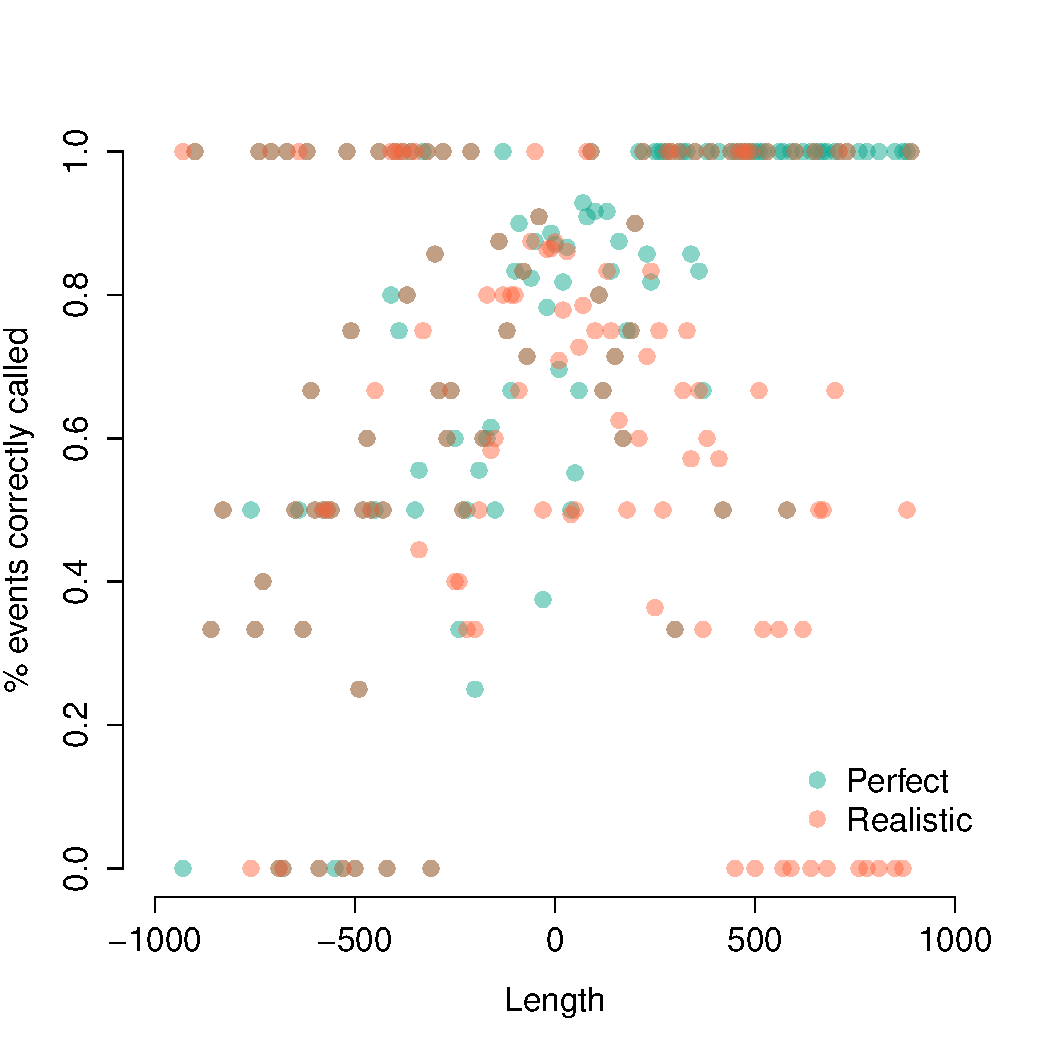
\includegraphics[width=\textwidth]{lengthHit-1}
  \caption{Event recovery as a function of event length}
  \label{fig:lengthHit}
\end{figure}
